\title{\textbf{Christian perspectives on sustainability: \\
		The need for numerical answers to philosophical questions.}}
\author{
		% Authors must be italicized.
        \emph{Jeremy Van Antwerp} and \emph{Matthew Kuperus Heun}%
\footnote{
Engineering Department, 
Calvin College,
Grand Rapids, MI, 49546, USA}
}

\documentclass[12pt]{article}

% CEC papers should be set in Times New Roman.
% https://tex.stackexchange.com/questions/153168/how-to-set-document-font-to-times-new-roman-by-command
% suggests the following.
\usepackage{mathptmx}             % For Times New Roman font (or a close approximation thereof).
\usepackage[margin=1in]{geometry} % For 1-inch margins all around.
\usepackage[document]{ragged2e}   % For left justification.
\usepackage{parskip}              % For double-spacing between paragraphs.
\usepackage{nopageno}             % To eliminate page numbers.
% For MLA bibliography. See https://www.ctan.org/pkg/biblatex-mla?lang=en for details.
\usepackage[american]{babel}
\usepackage{csquotes}
\usepackage[style=mla-new]{biblatex}
\addbibresource{JVAMKH.bib}

\usepackage{titlesec}             % To change formats of section titles, etc.
\titleformat*{\section}{\normalsize}
\titleformat*{\subsection}{\normalsize}
\titleformat*{\subsubsection}{\normalsize}
\titleformat*{\paragraph}{\itshape} % Set paragraph titles to italics
\usepackage{abstract}             % Set characteristics of the abstract
\setlength{\absleftindent}{0in}   % Do not indent left side
\setlength{\absrightindent}{0in}  % Do not indent right side
\usepackage{url}
\setlength{\parindent}{0in}       % Do not indent the 1st line of paragraphs.
\setlength{\parskip}{12pt}        % Instead, add space between paragraphs.
\renewcommand{\abstractnamefont}{\normalfont\normalsize} % Unbold and regular size
\renewcommand{\abstracttextfont}{\normalfont\normalsize} % Unbold and regular size
\date{}                           % To eliminate the date in the title

% To include graphics
\usepackage{graphicx}

% Commands for editing.

\usepackage{xcolor}            % For colored text
\usepackage[normalem]{ulem}    % For \sout command (strikethrough)

% From https://tex.stackexchange.com/questions/130623/crossing-out-using-different-colour,
% Change the \sout color to red
\newcommand{\redsout}{\bgroup\markoverwith{\textcolor{red}{\rule[0.5ex]{2pt}{0.4pt}}}\ULon}

% Use these versions to display changes.
\newcommand{\del}[1]{\textcolor{gray}{\redsout{#1}}}
\newcommand{\ins}[1]{\textcolor{red}{#1}}
\newcommand{\rev}[2]{\del{#1}\ins{#2}}

% Use these versions for a clean copy.
% \newcommand{\del}[1]{}
% \newcommand{\ins}[1]{#1}
% \newcommand{\rev}[2]{#2}



\begin{document}
	
\maketitle

\begin{abstract}
\noindent
%**** This is the abstract that I have on file. ---MKH ****
This paper presents a survey of Christian perspectives, from ancient to modern, on a
variety of sustainability-related topics such as stewardship of the natural world,
economic growth and technological change, energy, and human population. The emphasis is on
the development of thought and the lineage of ideas, with application to modern viewpoints
on current issues such as climate change, sustainable development, and human migration. We
review four modern strands
(eco-justice, stewardship, ``ecological spiritualities'', and consumptive economic prosperity) 
arising from four Christian traditions 
(Roman Catholicism, reformed Christianity, Eastern Orthodoxy, and conservative evangelicalism,
respectively),
leveraging a topology developed by Willis Jenkins \autocite{Jenkins:2008}.

The paper will cover a broad range of Christian thought and teaching in a digestible and
coherent format. It will serve as a supplement to a future engineering textbook on
sustainability challenges. Textbook chapters will provide a platform of background
knowledge to facilitate one-hour in-class discussions of several sustainability topics or
challenges. The conference presentation will highlight one area of Christian thought
(stewardship) and focus on piloting classroom discussion questions related to the theology
of sustainability.


% !!!! OBJECTIVE IS TO ACCURATELY SUMMARIZE THE FULL RANGE OF CHRISTIAN THOUGHT ON SUSTAINABILITY ISSUES.
% !!!  FOCUS IS ON 
% !!!! STRESS COMMONALITIES, NOTE DIFFERENCES

\end{abstract}


%%%%%%%%%%%%%%%%%%%%%%%%%%%%%%%%%%%%%%%%%%%%%%%%%%%%%%%%%%%%%%
\section{Introduction}
\label{sec:introduction}
%%%%%%%%%%%%%%%%%%%%%%%%%%%%%%%%%%%%%%%%%%%%%%%%%%%%%%%%%%%%%%

%\ins{We want to discuss eschatology somewhere.}

%\ins{We want to introduce engineering earlier in the paper.}

\ins{We need to signal early that we're not having the debate about whether
GW is happening or whether humans can cause large-scale environmental degradation.}

\ins{failure of our existing ethical frameworks, e.g., ethical review boards.}

The topic of sustainability is often organized into three categories: 
environmental, economic, and social. 
Environmental sustainability involves preservation of the nonhuman creation.
Economic sustainability refers to
the preservation and increase in value of human activities. 
In other words, not everything we do can lose money. 
 The notion of \emph{stewardship}, which originates in Genesis 1:28, is
foundational to Christian views on environmental and economic sustainability.
Social sustainability refers to relationships among humans: 
there should be justice, peace, order, and flourishing in human society. 
For Christians, the root of social aspects of sustainability
is the command to ``love your neighbor as yourself'' (Mt 22:39). 
Overarching these three areas of sustainability are 
concerns for human shalom and wellbeing.

Different Christian traditions understand the relationship 
between humans and the nonhuman creation differently, and
each tradition is informed by worldviews 
that are at times compatible and at other times discordant. 
Different Christian traditions have differing views 
on the economic and social themes of sustainability, too.
\ins{Christian understandings of the \emph{telos} of the created world
and eschatology inform sustainability choices.}
This paper explores the questions 
``How do Christians think about sustainability topics?'' 
and 
``Where do their views come from?'' 

\ins{Is is especially important the engineers, as creators and practitioners of technology, 
be aware of the sustainability challenges facing the world today, and, as Christian engineers,
be equipped to wrestled with the deep, complex, and interdisciplinary challenges associated
with transitioning to a sustainable society. Sustainability challenges have been called ``wicked problems'' %citation needed
because of their complex, interdisciplinary, and multifaceted nature. 
However, as we will show below, ``wicked'' is only the tip of the iceberg.
Sustainability challenges are hard to address because humans lack 
the philosophical and theological tools required to address them.}


The paper is organized as follows:
\ins{We briefly review Christian thought on the three areas of sustainability
in Sections~\ref{sec:economic}~and~\ref{sec:environmental}.
In Section~\ref{sec:personal_transportation}, 
%we apply the strands of Christian thought
%to a current sustainability issue,
%personal transportation vehicles,
we explore how Christian worldviews matter 
when sustainability issues are at stake
by evaluating, by example, a proposal to ban personal transportation vehicles
to improve the environment.
Section~\ref{sec:conclusions} concludes, and
the appendix lists additional questions/issues 
that need to be evaluated from a Christian perspective to achieve a sustainable future.}



%Things to add:
%\begin{itemize}
%  \item Utilitarian/Kantian ethics
%\end{itemize}

%2%%%%%%%%%%%%%%%%%%%%%%%%%%%%%%%%%%%%%%%%%%%%%%%%%%%%%%%%%%%%
\section{Economic and Social}
\label{sec:economic}
%%%%%%%%%%%%%%%%%%%%%%%%%%%%%%%%%%%%%%%%%%%%%%%%%%%%%%%%%%%%%%

\begin{figure}
\centering
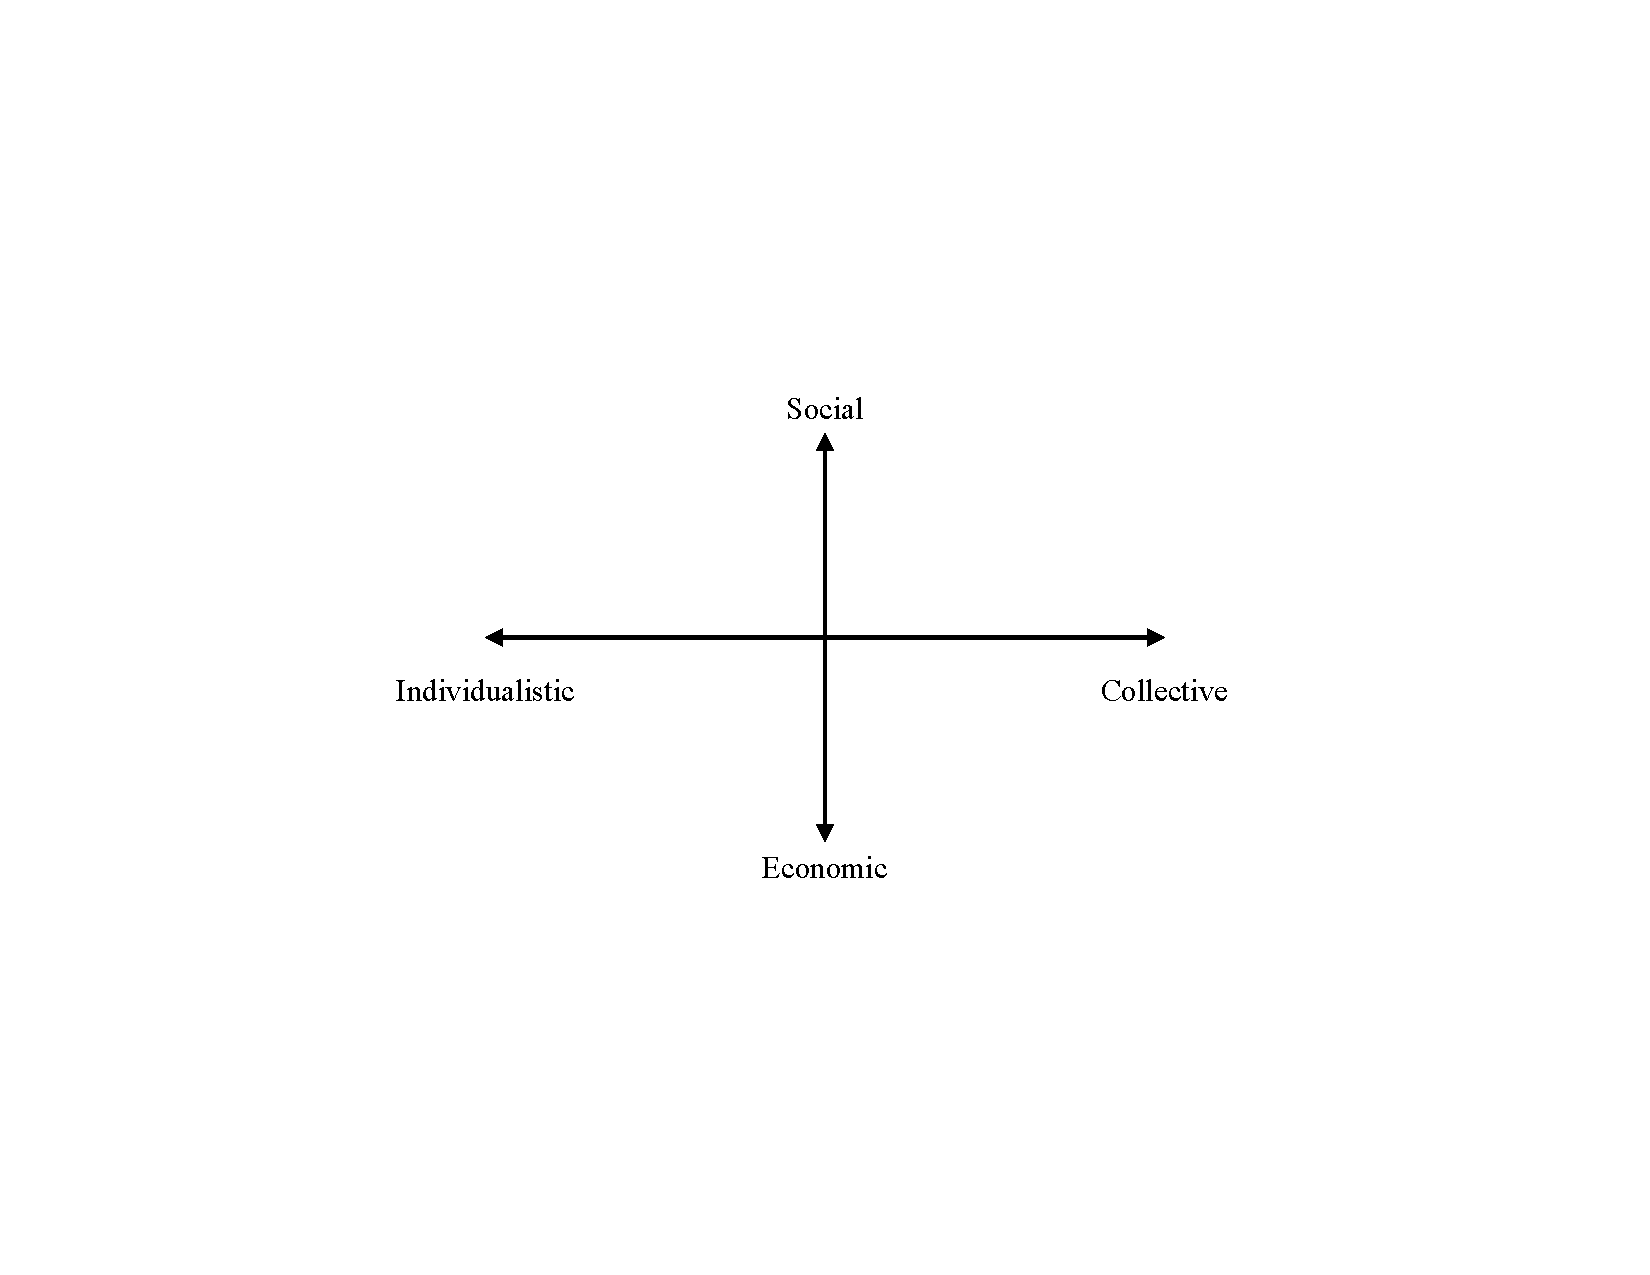
\includegraphics[width=0.65\linewidth]{figure_other/QuadAxes}
\caption{Axes for individualistic and collectivistic views on economic and social issues.}
\label{fig:axes}
\end{figure}

\begin{figure}
\centering
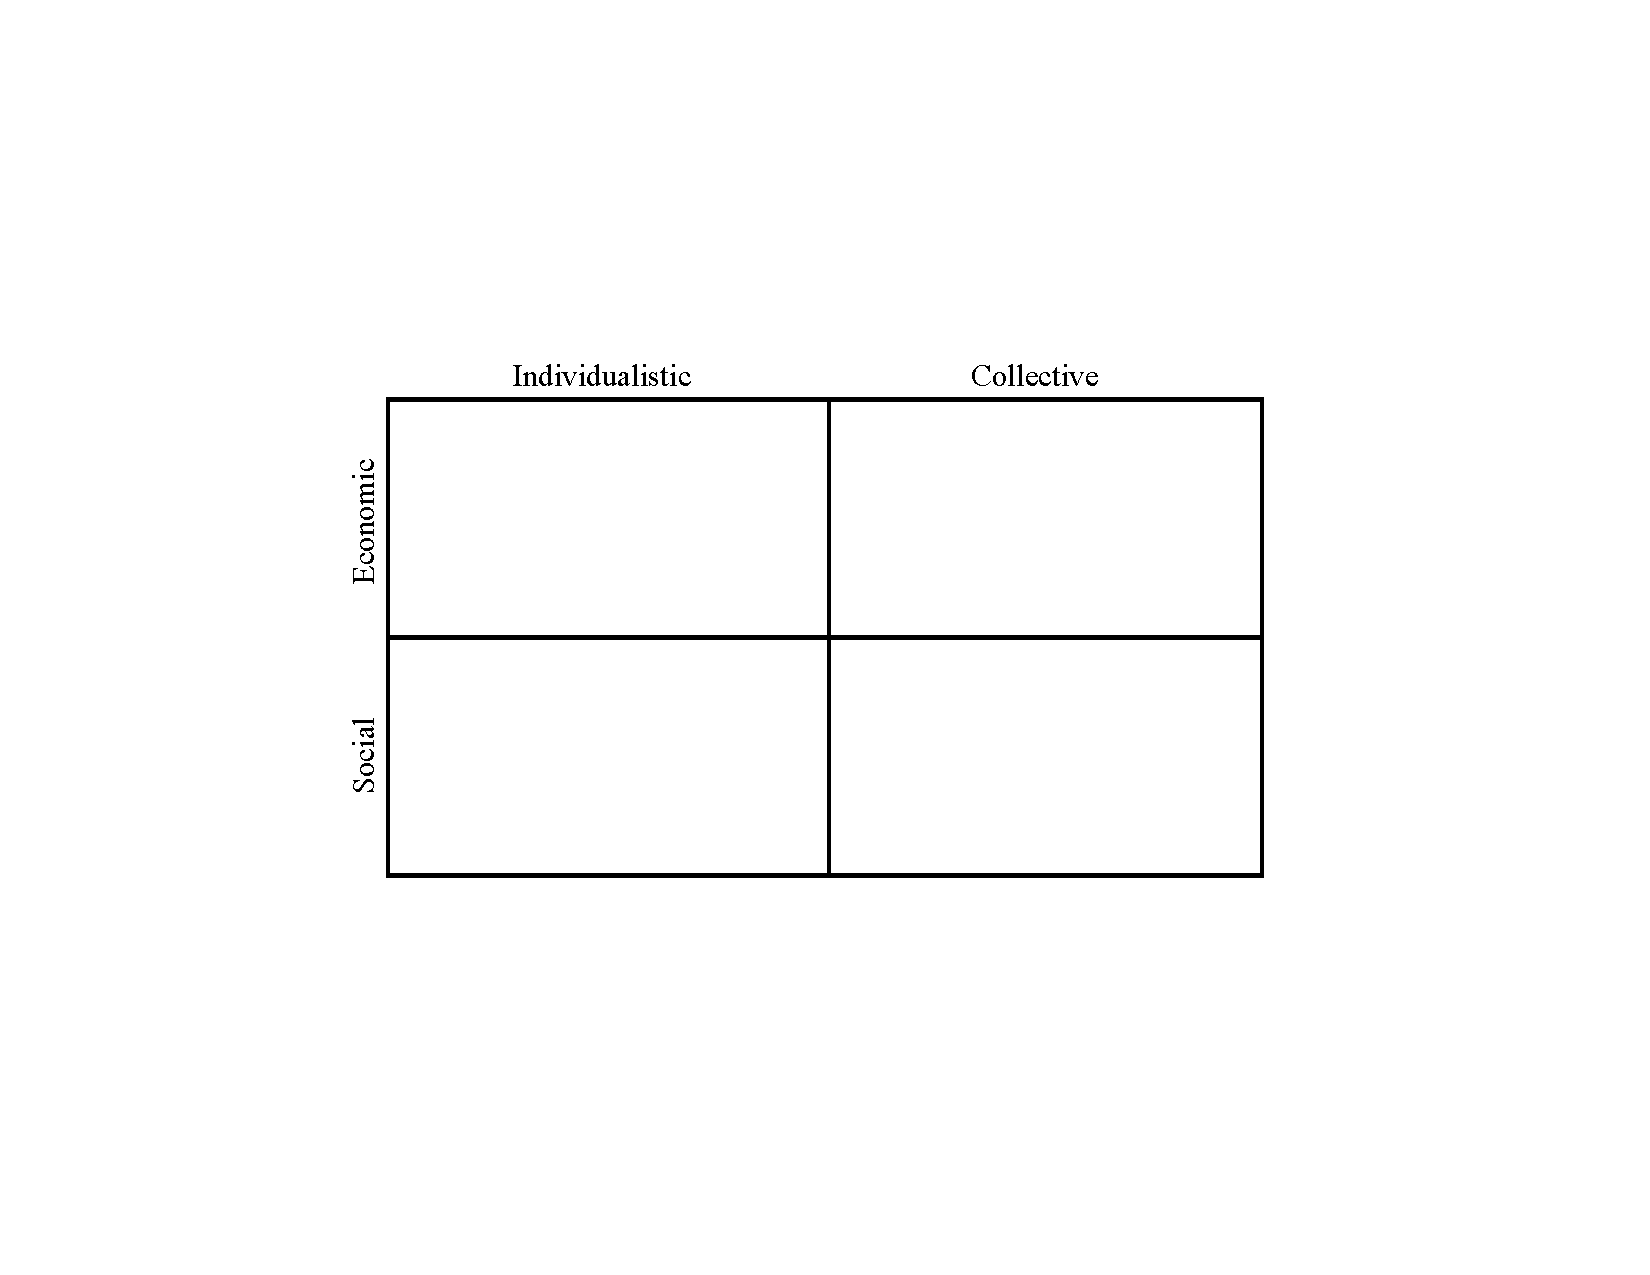
\includegraphics[width=0.75\linewidth]{figure_other/QuadTable}
\caption{Table for individualistic and collectivistic views on economic and social issues.}
\label{fig:table}
\end{figure}


Economics and politics (or ``the social'' aspects of sustainability) are inextricably linked. Biblical teaching on money
and justice are often recognized as two sides of the same coin, for instance in Micah 2:1-2, where the unjust deeds that
are denounced are economic in nature. Biblical teaching on economics and justice tends not to be in terms of a
systematic, over-arching theory, but rather in terms of individual interactions.
One exception to this pattern is the Old Testament sabbatical/jubilee system of canceling debt and returning property. 
In modern economic terms, canceling debts and returning property would serve to minimize 
\emph{income inequality} and ensure that there was uniform access to the \emph{means of production}.

From the first chapter of Genesis, the call to stewardship of all creation has
been understood by Christians to include money. The power of earthly resources to accomplish ``heavenly things'' is made
explicit in the parable of the shrewd (or dishonest) manager in Luke 16. To this end, the great majority of the Bible's
teaching on money relates to generosity to the poor. Numerous Old and New Testament passages instruct God's faithful to
give generously to the poor, the disadvantaged, and the marginalized, where ``giving'' is some combination of money
(traditionally called ``alms''), material goods (such as food or clothing), and justice or fairness.

One branch of Christian thought views wealth itself as a root of evil. This view goes beyond merely \emph{love} money
being the root of evil (I Tim 6:10). Proponents of the view that money itself is a source of evil would point to Jesus
telling the rich young man to sell all his possessions and give to the poor and Jesus' further comment that it is easier
for a camel to go through the eye of a needle than for a rich man to enter the kingdom of God (Mt 19:16-30, Mk 10:17-31,
Luke 18:18-30). At the other end of the spectrum of Christian thought, worldly wealth is seen as God's blessing, even an
indication of his favor (in a more extreme version of this view).

In terms of modern economic views, Christians hold a wide range of positions. Many Christian traditions advocate a
communal economic arrangement, in imitation of the early church (Acts 2:42-46). Examples range monastic orders such as
might be found in Roman Catholic or Eastern Orthodox traditions to the Hutterite and Bruderhof communities, which come
from an Anabaptist tradition. At the other end of the economic spectrum, many Christians advocate for an economic system
based on individual ownership and freedom of enterprise. Some key verses that support a more individual view include the
comments ``Didn’t it belong to you before it was sold? And after it was sold, wasn’t the money at your disposal?'' (Acts
5:4) and Paul's instruction that we should work to eat (2 Thes 3:10) and to share with those in need (Eph 4:28).
Thus, Christians hold a range of views from economic thought from communalistic to individualistic.

Likewise, Christian social perspectives can stress individual freedom, which we'll call ``liberal','' or collective behavior, which
we'll call ``collective.'' A liberal approach to providing for poor widows would be represented by the instruction that widows should be 
provided for, first of all, from their own families (1 Tim 5:4). 
The collective approach is represented by the group effort of caring for widows at the beginning of Acts chapter 6.
How Christian church denominations are organized is another example of this liberal-to-collective spectrum.
At the liberal end of the spectrum are ``independent'' bible churches. In the middle are denominations that follow a presbyterian form of church 
government. The local church in the presbyterian system has some autonomy but within the constraints of the broader 
denominational structure. The local churches also have a voice in the operation of the collective. At the collective end of the spectrum 
are denominations that use an episcopal form of church government. For example, the Roman Catholic church is very ``top down'' 
in how it operates.

We next show how the individualistic/communalistic economic perspective and the liberal/collective social (political) perspective
apply to a solving sustainability problems.

\ins{add 4-quadrant diagram?}

\subsection{Christian solutions to the tragedy of the commons}
\label{sec:totc}
The term ``tragedy of the commons'' was popularized by Hardin \autocite{Hardin68} 
and is used as a shorthand way of referring to
situations where there is equal and open access to a resource or pool of resources and it is in the rational self-interest of
every individual to maximize their use of the resource, even if this results in the net effect of destroying the
resource itself through over exploitation. This class of problems is recognized as ``having no technical solution.''
Instead, sustainable solutions are the result of social and/or economic policies. This section will examine several
Christian responses to the tragedy of the commons.

As originally stated, each herdsman had incentive to add more animals to his flocks grazing on the common land, since
the benefits (the extra animals) would accrue solely to him but the cost (degradation of the land) would be split between
all herders using the land for grazing. Moreover, since he knew that every other herder faced the same set of
incentives, it is rational to predict that the land will be ruined and that he should ``get while the getting is good.''
The ``tragedy'' lies in the ``remorseless working out of things.''

One communalistic solution to the tragedy of the commons is for all of the animals grazing on the commons to be common
property. Every member of the community would receive an equal share of the common herd (for example, cash value of the
meat raised at the end of the year). It would thus be in every individual's self-interest to maximize the \emph{total}
output, not just their own output. An individualistic solution is to charge each herder an increasing amount of rent for
each additional animal placed on the common land, which would create a financial incentive for each herdsman to keep
only a reasonable number of animals on the common land. A liberal social solution would be for each herder to be allowed
only a limited number of animals on the common land. A collective solution would be where an authoritative governing
board is set up to administer the common land. The board decides how many animals total are allowed and what proportion
of that total is allocated to each individual herdsman.

As we'll see below, many sustainability challenges are wholly or partly ``without technical solution'' and we need
Christian approaches to solving these problems.

%
%Wealth is a sign of God's blessing. 
%Personal property. Western of ``Christian'' concepts.
%The Enlightenment and the concept of personal freedom.
%Development of corporations.
%Theology of saving. Commerce, banking, financial trading.
%Roman Catholic response(s) to communism?
%Who owns land? Labor? Capital?
%
%% Quote from Wikipedia on Distributionism 
%% https://en.wikipedia.org/wiki/Distributism
%Distributism is an economic ideology asserting that the world's productive assets should
%be widely owned rather than concentrated.[1] It was developed in Europe in the late 19th
%and early 20th centuries based upon the principles of Catholic social teaching, especially
%the teachings of Pope Leo XIII in his encyclical Rerum novarum (1891) and Pope Pius XI in
%Quadragesimo anno (1931).[2][3][4] It views both capitalism and socialism as equally
%flawed and exploitative, and it favors economic mechanisms such as small-scale
%cooperatives and family businesses, and large-scale anti-trust regulations.
%
%Some Christian Democratic political parties have advocated distributism in their economic
%policies.
% end quote

% In this issue, Nathan Schneider writes about Pope Francis’s economics. Here, he
% recommends five books of Catholic thought that display strikingly similar concerns to
% those of secular activists today. Each one emphasizes the wisdom of ordinary people. “In
% church each week,” Schneider says, “I learn Catholic economics from the diversity of
% classes and colors who meet under the image of an executed radical.”
%  https://www.thenation.com/article/classics-of-catholic-economics/

% from ENGR 184 lecture slides: 
% ``socially desirable and economically viable.''
% Economic: profit, cost savings, economic growth, R\&D
% Social: standard of living, education, community, equal opportunity. These combine to be business ethics, fair trade, women's rights.
% Economics refers to the whole community impact, not just a company's bottom line.
% social is fair business practices to labor and the community (whatever that means).
% Economics is the social science that seeks to describe the factors which determine the production, distribution, and consumption of goods and services.
% Food production, distribution, quality -- relates to land use and water consumption (3 models of agriculture: what's ``most efficient?'')

%Suffering and justice. Care for the poor. 
%Kings, democracy, dictators.
%Medicine, water, health care. What are ``rights?''
%What are the means of redress?
%Just war? just use of ``power?''
%Sphere sovereignty and the role of government? Church? family ... school...


%1%%%%%%%%%%%%%%%%%%%%%%%%%%%%%%%%%%%%%%%%%%%%%%%%%%%%%%%%%%%%
\section{Environmental}
\label{sec:environmental}
%%%%%%%%%%%%%%%%%%%%%%%%%%%%%%%%%%%%%%%%%%%%%%%%%%%%%%%%%%%%%%

\ins{Add first action for sustainability? The weakness or pitfall of each approach. (for instance, lack of information?)
Need to add in for each worldview, discussion question 13, what is the purpose of the natural world?}

Willis Jenkins' book \emph{Ecologies of Grace} \autocite{Jenkins:2008}
provides a topology of Christian thought regarding the 
nonhuman creation and the
environmental aspect of sustainability.
He identifies three schools of thought:
stewardship, 
eco-justice, and 
ecological spirituality,
which loosely correspond to 
Reformed (or evangelical protestant), 
Roman Catholic, and 
Eastern Orthodox 
traditions.
To Jenkins' three, we add a fourth:
consumptive economic prosperity and
the conservative evangelical tradition. 
These four schools of thought 
span a wide range of Christian stances toward the nonhuman creation
and 
consequently outline a range of possibilities 
for Christian responses to environmental issues
and environmental sustainability concerns more broadly.
One way to begin unpacking the four schools of thought 
is to identify a keyword for each:
\emph{redemption} for stewardship, 
\emph{sanctification} for eco-justice,
\emph{deification} for ecological spirituality, and
\emph{resilience} for consumptive economic prosperity.

%..............................
\paragraph{Redemption} 
\label{sec:redemption}
%..............................

The stewardship school of thought in the Reformed tradition
emphasizes that all of human existence
is a response to God's redemptive acts
and God's providence to humans.
Knowing God leads to vocational responsibility 
to care for nonhuman creation,
which is the means by which God provides for humankind 
% For some reason, we need to include this citation twice to get both author and page number to appear.
(\textcite{Jenkins:2008} \textcite[19]{Jenkins:2008}). 
Thus, all human work to care for the creation 
is seen as service to the Creator
out of gratitude for redemption (\textcite{Jenkins:2008} \textcite[77]{Jenkins:2008}).
\emph{Earthkeeping} \autocite{Wilkenson:1980aa} provides a cogent summary
of the importance of redemption for Reformed Christians doing creation care.

%..............................
\paragraph{Sanctification} 
\label{sec:sanctification}
%..............................

The eco-justice school of thought in the Roman Catholic tradition
emphasizes that God's grace reveals the creation's 
inherent integrity \autocite[19]{Jenkins:2008}, 
giving it natural value and inherent moral standing~\autocite{Joldersma:2019}. 
Thus, Christians must respect creation's inherent value and 
respond to its moral standing in all activities.
If the nonhuman creation can't speak for itself, 
we must speak for it and defend it when necessary.
The \emph{Laudato Si} encyclical \autocite{Pope-Francis:2015aa} 
is a clear enunciation of Roman Catholic thought
on environmental sustainability issues.

%..............................
\paragraph{Deification} 
\label{sec:deification}
%..............................

The deification school of thought in the Eastern Orthodox tradition
highlights the union between all of creation and God.
This view holds that there is a radical, integral relationship between humans and 
the nonhuman creation~\autocite[93]{Jenkins:2008}.
The speech ``To Commit a Crime Against the Natural World Is a Sin'' 
\autocite[133-136]{Bartholomew-I-of-Constantinople:2011aa}
provides an excellent summary of the Eastern Orthodox view
on the nonhuman creation.

%..............................
\paragraph{Resilience} 
\label{sec:resilience}
%..............................

The resilience school of thought in the conservative evangelical tradition
holds that the nonhuman creation is resilient, robust, and self-correcting.
Furthermore, its well-being is assured by God.
In addition, human well-being is paramount. 
Thus, humans are to be consumers of the nonhuman creation 
to provide economic prosperity and
lift people out of poverty.
Documents from the Cornwall Alliance 
provide a summary of conservative evangelical thinking on creation care issues
\autocite{Cornwall:2006aa}.

% Natural world is inherently good.
% Natural world should be conquered and ruled over (in part, because it is `red in tooth and claw.')

% Include table with links to denominational statements on climate change, whaling, conservation, pollution, wilderness?

% *** Here is a URL that shows how to convert a .csv file into a LaTeX table.
%
% \url{https://www.latex-tutorial.com/tutorials/pgfplotstable/}
%
% Here is a link to the Google sheet.
%
% {\tiny \url{https://docs.google.com/spreadsheets/d/1OD7LFbCU0Rdv3-vAM0MbIBd4hkEwxwY2FtP0XfvAU_M/edit#gid=0}}

%%%%%%%%%%%%%%%%%%%%%%%%%%%%%%%%%%%%%%%%%%%%%%%%%%%%%%%%%%%%%%
\section{Application: personal transportation}
\label{sec:personal_transportation}
%%%%%%%%%%%%%%%%%%%%%%%%%%%%%%%%%%%%%%%%%%%%%%%%%%%%%%%%%%%%%%

% needs to somehow address the framework by which we make choices. I want to get at the utter failure of current and past modes of thinking
% in allowing us to address sustainability-related questions.
Far from being esoteric or merely philosophical, 
the impact of worldview on sustainability issues and behavioral choices 
is both crucially important and entirely practical. 
Thus, it is \emph{essential} that engineers consider worldviews
when examining choices and tradeoffs related to sustainability.
This section considers, as a practical example, the effects of different Christian approaches
to the economy and societal structures (Section~\ref{sec:economic}) and
to the nonhuman creation (Section~\ref{sec:environmental})
on a sustainability-related policy question, 
namely whether to ban vehicles for personal transportation.

In 2017, the United States emitted 5.14 billion metric tons equivalent of greenhouse gases, 
of which, about 1.8 billion tons (35\%) were from petroleum used for transportation \cite{EIA2017}.
Consider a proposed ban on personal transportation vehicles.
Commercial vehicles are not addressed by the proposed ban. % is that fair? what about rental cars?

The alternative to the proposed ban is to do nothing. 
Under this ``null hypothesis,'' 
significant amounts of greenhouse gasses would be added to the atmosphere 
at ever-increasing rates. \ins{Do we need to explain ever-increasing rates?}
Enacting the proposed ban would eliminate a (major) category 
of greenhouse gas emissions and 
would be a step on the road toward sustainability
and would, presumably, avoid future costs for climate change adaptation.
However, the proposed ban would involve massive monetary costs in the near-term. 
Billions of dollars per year would be required. 
One estimate \ins{citation needed} is that it would require between 7 and 14\% of GDP annually 
over 20 years to achieve a fully-renewable transportation infrastructure.

Emplacing a fully-renewable transportation infrastructure 
would displace or require thorough transformation of many existing industries, including 
the automobile industry, 
the liquid petroleum distribution industry, and
the electricity generation and distribution industries,
to name a few.
Disruptions in those industries 
would cause massive social disruptions 
as jobs are lost.
Therefore, a large-scale job retraining effort would be necessary.

The proposed ban would have massive implications for real estate values 
and patterns of land use. 
Presumably, rural living would be much more difficult if the proposal were enacted,
whereas urban dwellers could avail themselves of extensive public transit networks.

Questions about the legality of a ban on personal transport vehicles would surely arise.  
Even for the benefit of the long-term survival of life on planet Earth,
would we make such a draconian decree? 
Is it even ethical to do so?


%++++++++++++++++++++++++++++++
\subsection{Evaluating tradeoffs}
\label{sec:evaluating_tradeoffs}
%++++++++++++++++++++++++++++++

Implementing the proposed ban on personal transport vehicles
will involve tradeoffs among the dimensions of sustainability, 
environmental, economic, and social factors.
Decisions on tradeoffs are necessarily informed by worldviews,
many of which are briefly described 
in Sections~\ref{sec:economic} and~\ref{sec:environmental}.
In this subsection, 
we use the proposed ban to explore how Christian worldviews matter 
for tradeoffs when sustainability issues are at stake.
That is, how do each of the Christian traditions 
\ins{(Is Christian traditions the right way to discuss these ideas?)} 
discussed in this paper 
evaluate tradeoffs among environmental, social, and economic factors?
We briefly summarize each tradition below.
\ins{again, maybe want to merge with sections above to avoid repetition. What are the weaknesses of each approach?}

%..............................
\paragraph{Individualistic} 
\label{sec:example_individualistic}
%..............................

Stuff here about the individualistic approach to economic and social aspects of sustainability.


%..............................
\paragraph{Collective} 
\label{sec:example_collective}
%..............................a

Stuff here about the collective approach to economic and social aspects of sustainability.


%..............................
\paragraph{Reformed (stewardship)} 
%..............................

The stewardship approach emphasizes the human responsibility 
to care for the nonhuman creation
as a response to God's redemptive actions.
It acknowledges that tradeoffs 
are present in every policy and in every decision. 
So, in an engineering sense, 
Christian environmental stewardship could be considered an optimization problem
in which policies that bring about the most good 
are to be preferred.
Who decides what goods matter most is important, and 
all voices should be heard on this matter.
Ignoring or disregarding voices is dangerous,
since injustices could result. %need perfect economic and environmental information?
Humans will be persuaded on the right course of action
for sustainability policies by weighing the tradeoffs 
among environmental, economic, and social factors.
\ins{Here is an example of where imperfect information, in both an engineering sense and an economic sense, would bite you big time.}

%..............................
\paragraph{Roman Catholic (eco-justice)} 
%..............................

The eco-justice approach is based upon the moral standing of the nonhuman creation,
meaning that the nonhuman creation itself must be given a voice. 
To properly evaluate sustainability tradeoffs,
someone must be empowered to speak for the nonhuman creation and 
give voice to unjust and unfair aspects of policies and decisions
that have implications for sustainability and the nonhuman creation.
Humans will pursue the right course of action on sustainability issues
when someone speaks eloquently and forcefully for the 
those who can't speak for themselves, including the nonhuman creation. 

%..............................
\paragraph{Eastern Orthodox (ecological spirituality)} 
%..............................

The primary departure point for ecological spirituality is the radical connection between 
the creator and the creation.
Consequently, and by virtue of both owing their existence to the creator, 
there is a radical connectedness among all human and nonhuman creatures in the creation.
Because of this radical connection between humans and the nonhuman creation, 
any good done to the environment is a good done to humans, 
and praiseworthy. 
Conversely, any environmental harm is a harm to humans and sinful. 
We should always be doing right by ourselves and the environment 
to please the God of us all.
In ecological spirituality, 
tradeoffs between the environmental and social realms of sustainability
fade into the background.
And because the economy is a way of organizing social relationships and structures,
tradeoffs between the environmental and economic are minimized, too.

%..............................
\paragraph{Conservative Evangelical (consumptive economic prosperity)} 
%..............................

In this worldview, 
any environmental degradation caused by humans will be fixable,
given sufficient economic resources and the guidance of the free market's invisible hand.
People with the consumptive economic prosperity worldview
will note that a ban on all personal transport vehicles 
will likely lead to decreased economic prosperity,
as some people will no longer be able to work,
commute times will increase for others, and 
commerce will slow. 
A reduction in economic prosperity will, ultimately, be bad for the environment, because
we will have fewer economic resources with which to address environmental damage.
Thus, those whose focus is consumptive economic prosperity will 
be unlikely to support the proposed ban on personal transportation vehicles.


%++++++++++++++++++++++++++++++
\subsection{A conundrum}
\label{sec:conundrum}
%++++++++++++++++++++++++++++++

The proposed ban on personal transportation vehicles
implicitly accepts a conundrum: 
you can't have personal transport vehicles and a flourishing environment. 
In this subsection, we consider several questions about the conundrum and 
explore ways out of the conundrum,
guided by the worldviews discussed above.
\ins{Need a transition here.
Maybe another way to say it:
we don't actually do what the leading paragraph promises.
The worldviews are not applied consistently.}

%..............................
\paragraph{What assumptions are behind the conundrum?} 
%..............................

The proposed solution assumes that all personal transport vehicles degrade the nonhuman creation. 
The proposed solution does not allow for variation in environmental damage
from different modes of transport or different types of vehicles.

%..............................
\paragraph{Can you think of alternative policies that break free from the conundrum and solve the dilemma?} 
%..............................

It may be possible to incentivize any number of low-impact vehicles, including 
bicycles and renewable energy vehicles.
Policies to incentivize adoption of 
mass-transit (subways and busses) or shared transit (Lyft and Uber)
could allow societies to meet transport needs with significantly less environmental impact 
per person-km.

But tradeoffs exist. 
There are financial costs to changing the transportation infrastructure to low-impact vehicle technologies
or away from personal to mass-transit solutions. 
There will be social costs to changing the transportation infrastructure as well.
Relationships and employment may be disrupted by changes in the availability of personal transport vehicles,
especially if substitutes are of lesser quality or availability.
Converting to a renewable-energy personal transportation infrastructure 
might imply land-use changes, 
requiring significant amounts of space for solar and wind renewable electricity production,
not to mention storage needs. 
Will land-use changes impinge on the ``freedom'' or rural life 
or increase the density of urban living?

%..............................
\paragraph{How might Christian worldviews shape perceptions of these tradeoffs?} 
%..............................

Perceptions of the desirability and advisability of choices implied by these tradeoffs 
will be shaped by the Christian worldviews discussed above.

\ins{Add something from collective approach here.}

\ins{Add something from individualistic approach here.}

For example, stewardship concerns may indicate deep study of alternatives, 
weighing weigh costs and benefits in the environmental, economic, and social realms
to discover the best way to manage the human and nonhuman elements of creation.
Study and deliberation will be in order as debates over the numeraire for comparisons arise.
Those informed by an eco-justice worldview may want to evaluate 
differential benefits and costs of a transportation system overhaul.
To whom will benefits and costs accrue? 
Which people groups will benefit most and least? 
Which portions of the nonhuman creation will benefit or be harmed? 
Those in the deification school of thought might be concerned 
about loss of quality of personal connections 
among people due to transportation system disruption
and advocate for policies that ensure transportation system changes 
are coupled with ways to increase the connectedness that people
feel toward the nonhuman creation.
Those with a resilience mindset may be likely to disfavor 
large-scale changes to the transportation infrastructure 
on the grounds that the financial cost of a transportation system overhaul would be burdensome,
without much regard for any environmental benefits, 
because the Earth system is resilient anyway.



% Maybe different rules for different places?
% Techno-optimism (technocism?)
% posits there is a way to solve all problems with sufficiently advanced technology.
% What would be the (socialism?) way?---there's a way to solve every problem
% with a sufficiently advanced society.




%%%%%%%%%%%%%%%%%%%%%%%%%%%%%%%%%%%%%%%%%%%%%%%%%%%%%%%%%%%%%%
\section{Conclusions}
\label{sec:conclusions}
%%%%%%%%%%%%%%%%%%%%%%%%%%%%%%%%%%%%%%%%%%%%%%%%%%%%%%%%%%%%%%

% one conclusion that we've talked about is the need for a theology that addresses corporate sin/responsibility for the environment.
% How does, for instance, covenant theology lead us to sustainability?

The purpose of this paper is to explore how
Christian worldviews matter 
when sustainability issues are at stake. 
The example discussed in Section~\ref{sec:personal_transportation} shows that
Christian worldviews can and do 
both inform responses to sustainability issues
and affect assessments of policy tradeoffs.

In reviewing Sections~\ref{sec:environmental}--\ref{sec:personal_transportation},
it becomes clear that there is an urgent need for a theology 
that addresses human effects on the nonhuman creation.
This theology should provide guidance for daily life and 
for corporate decision- and policy-making on several axes:
economic gain vs.\ environmental harm, 
individual harm vs.\ corporate good, 
benefits to the current generation vs.\ future generations,
environmentally harmful but convenient solutions vs.\ environmentally benign but inconvenient solutions, 
dollar-quantifiable goods and harms vs.\ non-quantifiable goods and harms,
costs and benefits that accrue to an individual vs.\ a group
or a group vs.\ an individual, etc.

Indeed, there is much work to be done.


\appendix

%%%%%%%%%%%%%%%%%%%%%%%%%%%%%%%%%%%%%%%%%%%%%%%%%%%%%%%%%%%%%%
\section{Discussion questions}
\label{sec:discussion_questions}
%%%%%%%%%%%%%%%%%%%%%%%%%%%%%%%%%%%%%%%%%%%%%%%%%%%%%%%%%%%%%%

Section~\ref{sec:personal_transportation} demonstrated application of 
the Christian worldviews discussed in Sections~\ref{sec:economic} and~\ref{sec:environmental}
to an environmental sustainability issue and a hypothetical policy prescription.
In this appendix, we provide several additional issues and policy prescriptions 
to which Christian worldviews could be applied.
The issues and policy prescriptions are presented in the form of discussion questions
for use in classrooms or with small groups.
%
\ins{I suggest we merge this  list into the Appendix}
\begin{itemize}
\item{What are the economic sustainability issues we want to address? How do we want to address them?}
\item{Global poverty and other ills associated with it like lack of access to clean water and food insecurity.}
\item{The concept of continual economic growth based on extractive consumption.}
\item{Carbon tax}
\end{itemize}

\begin{enumerate}
	
  \item In Section~\ref{sec:personal_transportation}, 
        a proposed solution to address environmental degradation caused by 
        personal tranport vehicles is banning all personal transport vehicles.
		%
		\begin{itemize}

		  \item The proposed solution might solve an environmental problem. 
		        But it may cause social and economic problems. What are they?

		  \item Suppose reducing the number of personal transport vehicles 
		        results in job losses for auto industry employees. 
				How should Christians respond to unemployment that results 
				from something ``good,'' like saving the environment? 

		  \item	Should there be a ``social safety net?'' If so, how big should it be? 
		  
		  \item Are your responses informed by your Christian worldview or your political orientation?  
		  
		  \item Does your answer depend on whether the job losses are the result 
		        of technical innovation (``progress'') or new regulations
				that prohibit something or reduce ``freedom?''
				
		\end{itemize}

  \item An alternative to banning all personal transportation vehicles would be banning 
        fossil fuel (FF) personal transportation vehicles. 
		An alternative to FF personal transportation vehicles is electric personal transportation vehicles
		that are manufactured, operated, and disposed using renewable electricity.  
		
		\begin{itemize}

		  \item How equivalent do FF and electric vehicles need to be before banning FF
		        personal transportation vehicles would be acceptable?
		
		  \item Would there be value to maintaining some FF personal transportation vehicles 
		        as a historical artefact? 

		\end{itemize}
		
  \item Banning all personal transport vehicles might be considered a ``clean'' or ``ideal'' policy option.
        Other policy options could be classified as pragmatic, 
		e.g.\ improving efficiency of personal transport vehicles.
		How should Christians navigate the space between ideal and pragmatic policy proposals? 
		Give examples.

  \item The transportation system (all modes, not just personal transportation vehicles) 
        provides economic value and connects people. 
        But it also causes CO$_2$ to be emitted in the manufacture, use, and disposal 
		of all vehicles (planes, trains, and automobiles). 
		We must reduce the CO$_2$ intensity of transport to move toward a sustainable future. 
		Air travel is more CO$_2$-intensive than automobile transport (per-person-km). 
		Thus, it is proposed that all air travel be banned.

		\begin{itemize}

		  \item Should we ban air travel? 
		        Why or why not? 
				Are there ethical aspects to this question or 
				only technical/practical aspects? 

		  \item In developing policies regarding air travel, whose opinion should we respect? 
		        Experts? Novices? 
				Technologists? Generalists? 
				Corporate executives? Blue collar workers?
				
  		  \item This policy question gets at several “axes” of tradeoffs and policy-making:
		        economic gain vs.\ environmental harm, 
				individual harm vs.\ corporate good, 
				benefits to current generation vs.\ future generations, and 
				environmentally harmful but convenient (e.g., jet airliners) vs.\ 
			    environmentally benign but inconvenient (e.g., blimps).
				How would each of the Christian worldviews discussed in Sections~\ref{sec:environmental}
				and~\ref{sec:economic} assess tradeoffs on these axes?
				
		\end{itemize}
		
  \item How would Christians holding the worldviews discussed 
        in Sections~\ref{sec:environmental} and~\ref{sec:economic} 
		respond to the following policy proposals
		for addressing climate change?
		%
		\begin{itemize}

		  \item Taxation of fossil fuel \emph{production}. using the proceeds to 
		        convert all energy infrastructure to renewables
		  
		  \item Taxation of fossil fuel \emph{consumption}, using the proceeds to 
		        convert all energy infrastructure to renewables

		  \item Stimulation of economic growth to create excess wealth to be applied 
		        in some proportion to environmental restoration, poverty alleviation,  
				or society-wide relationship counseling

		\end{itemize}
		%
  \item ``Environmental'' is only one dimension of sustainability. 
        Tradeoffs often exist among ``environmental,'' ``social,'' and ``economic'' 
		aspects of sustainability. 
		How would each Christian worldview discussed in the paper respond to the following tradeoffs?
		%
		\begin{itemize}

		  \item Long-term employment losses due to climate-change-caused flooding vs.\ 
		        short-term employment retention for coal miners

		  \item **** More here? **** 

		\end{itemize}
		%
  \item Any policy-driven change, 
        such as reducing carbon emissions by banning personal transport vehicles, 
		results in consequences that have 
		\emph{direct} dollar-measurable impacts 
		(such as increased personal cost per mile traveled),
		\emph{indirect} but still dollar-measurable consequences 
		(such as reduced CO$_2$ output), and 
		consequences that \emph{aren't} measurable in dollars 
		(such as an aesthetic impact on the landscape). 
		Economic cost-benefit analysis converts all social and environmental costs 
		to dollars, thereby providing a consistent numeraire and allowing direct comparisons
		among environmental, economic, and social effects. 
		%
		\begin{itemize}

		  \item How should Christians evaluate choices among 
		        policy solutions whose impacts are dollar-quantifiable
		        policy solutions whose impacts are \emph{not} dollar-quantifiable?

		  \item Similarly, Pareto optimality is used to conceptualize choices in a multiobjective environment. 
                How do Christians think about tradeoffs under Pareto optimality? 
		  
		  \item Should we be so mathematical in our decision making?
		  
		  \item How do/should Christian assessments of tradeoffs change 
				%
				\begin{itemize}

				  \item when cost and benefits fall to different (groups of) people? 

				  \item when many benefit at the expense of a few? 
				  
				  \item when few benefit at the expense of the many? 
				  
				  \item when benefits and costs accrue to different generations? 
				  
				\end{itemize}
				
		  \item Does the size of the benefit/cost matter? 
		  
		  \item Does the number of people in the group matter? 
		  
		  \item Are there guidelines on what’s a ``big enough'' difference to matter? 
		  
		  \item Possible frameworks within which to consider these questions include 
		        eminent domain, corporate profit vs.\ air pollution, 
				aquifer depletion, species extinction, and climate change. 		  
		  %
		\end{itemize}
		
  \item What is the Christian solution to the tragedy of the commons (Section~\ref{sec:economic})?

  % Propose deleting, because little has been said about population in the paper, 
  % and this questions appears "out of nowhere".
  % \item How are population growth and control different?
  %       What are Christian perspectives on each?
        
  \item Both the Old and New Testaments teach that Christians should work to eliminate poverty. 
        How do we respond to the observation that alleviating poverty increases economic consumption, 
		which has negative environmental consequences?
		
  \item A Brazilian farmer argues that he/she needs to make a living. 
        Can he/she create another subsistence farm in the Amazon rainforest?  
		What is the value of ``wilderness?''
		
  \item Which Christian tradition discussed in Sections~\ref{sec:environmental} and~\ref{sec:economic}
        resonates with you personally? Why? Which aspects of other Christian traditions do you embrace? Why?

  % Propose deleting because there are several other questions that get at temporal aspects
  % of tradeoffs.
  % \item What is the Christian approach to thinking about tradeoffs
  %       between long-term versus short-term effects?

  % Propose deleting, because many other questions address this tradeoff.		
  % \item Likewise, what's a Christian approach to thinking about tradeoffs in different areas
  %       (for instance, human well being versus the environment)?
		
  \item What is the purpose of the Creation? The natural world?

  \item What is aspects of economic sustainability are most important to a Christian?
  
  \item Why are disruptions from technological innovations seen as positive changes while disruptions from regulations seen as negative? 
  How does your view of justice influence your view of regulations?

\end{enumerate}

% Is anybody “doing theology” in this space?



\printbibliography


\end{document}